\documentclass[a4paper,12pt]{article}

\usepackage[utf8]{inputenc}
\usepackage[style=authoryear,backend=biber]{biblatex}
\usepackage[a4paper, margin=2.5cm]{geometry}

\usepackage{amsmath}
\usepackage{amsfonts}
\usepackage{amssymb}
\usepackage{graphicx}
\usepackage{wrapfig}
\usepackage{wasysym}
\usepackage{float}
\usepackage{pgfplots}

%\usepgfplotslibrary{external}
%\tikzexternalize
\graphicspath{ {./images/} }

\pgfplotsset{compat=1.18}
\renewcommand{\baselinestretch}{1.5}
\renewcommand*\contentsname{Table Of Contents}
\addbibresource{bibliography.bib}

\newcommand{\ResearchQ}{To what extent does changing the length of a circular cantilever beam affect its resonant frequency, and how well can the theoretical model predict this relationship?}


\begin{document}

\begin{titlepage}
    \begin{center}
        \vspace*{1cm}

        \textbf{Investigating Factors Affecting the Resonant Frequency of Cantilever Beams}\\

        \vspace{.5cm}
        \textbf{Research Question:}
        \ResearchQ

        \vspace{0.5cm}
        International Baccalaureate Physics Extended Essay

        \vfill

        \vspace{0.8cm}

        Word Count:744


    \end{center}
\end{titlepage}

\pagenumbering{Roman}

% Table of Contents
\tableofcontents
\addcontentsline{toc}{section}{Table Of Contents}
\pagebreak

\begin{abstract}
\addcontentsline{toc}{section}{Abstract}

    Write something here
\end{abstract}
\pagebreak

\pagenumbering{arabic}

\section{Introduction}%500rq have 211, maybe 250 more?

Cantilever beams, seemingly simple elements used in construction where one end of a beam is solidly attached and the other loose, has played a major role in engineering, historically they were used for purely mechanical structures such as buildings, cranes and balconies.
\autocite{BuildingConstructionBook}\\
While the use of such simple elements is still common in traditional construction, their utility expands far beyond macroscopic architecture, Nowadays cutting edge technology such as MEMS(micro-electromechanical) systems which integrate mechanical systems with electronics in a microscopic level, use such structures as well, microscopic cantilever beams are being used as inertial sensor in gyroscopes to sense tiny acceleration forces.
\autocite{MemsBook}%Analysis and Design Principles of MEMS Devices

I was fascinated to learn that such simple structures lie at the core of technologies we take for granted today. This pushed me to further investigate their functionality and their dynamic properties. My research question is ``\ResearchQ'' and
I aim to determine how the length of the beam and the initial energy loaded into the beam will affect the frequency that the beam naturally vibrates at when excited using pure mathematics, Finite Element Analysis and Experimentally.
As shown in \eqref{eqn:theory}, I am expecting to see the frequency is inversely proportional to the square of its length, and to see no relationship between the frequency and the initial energy load.

\begin{align}%eqn:theory
\label{eqn:theory}
\begin{split}
f_{n}\propto \frac{1}{l^{2}}
\\
f_{n}\not\sim E_{initial}
\end{split}
\end{align}






\section{Background Information}%600, 400 left
    \subsection{Fourier Transform} \label{FT}
    The fourier Transform is a
    \pagebreak
    \subsection{Finite Element Method}\label{FEM}%208rn, "done"
    In engineering, it is common to be faced with partial differential equations(PDE), these equations are usually complex and are computationally intense to calculate, for example, calculating heat transfer, fluid flow, or in the case of this paper, non-rigid bodies.
    The Finite Element Method(FEM) is a way method to estimate the result of the PDE, by dividing the continuous space of the problem into smaller, discrete parts called finite elements.

    The collection of the finite elements is known as the mesh. By dividing the space, analysis within each element becomes simpler, and later combined to get an estimation, this allows the computation of the differential equations to be computationally simpler. As this is a method of estimation, the results are not always accurate, to get the estimate closer to reality, the mesh resolution is increased at the cost of compute time.\autocite{FEABook} \\
    The use of this method of engineering analysis is commonly known as Finite Element Analysis(FEA) and will be used as a virtual experiment in \ref{FEA} to simulate the cantilever beams natural frequency.
    As this method allows to simulate deformation of bodies, this tool is generally built into Computer Aided Design(CAD) suites and Onshape, a cloud based CAD suite will be used in this paper.\\
    \begin{figure}[b]
    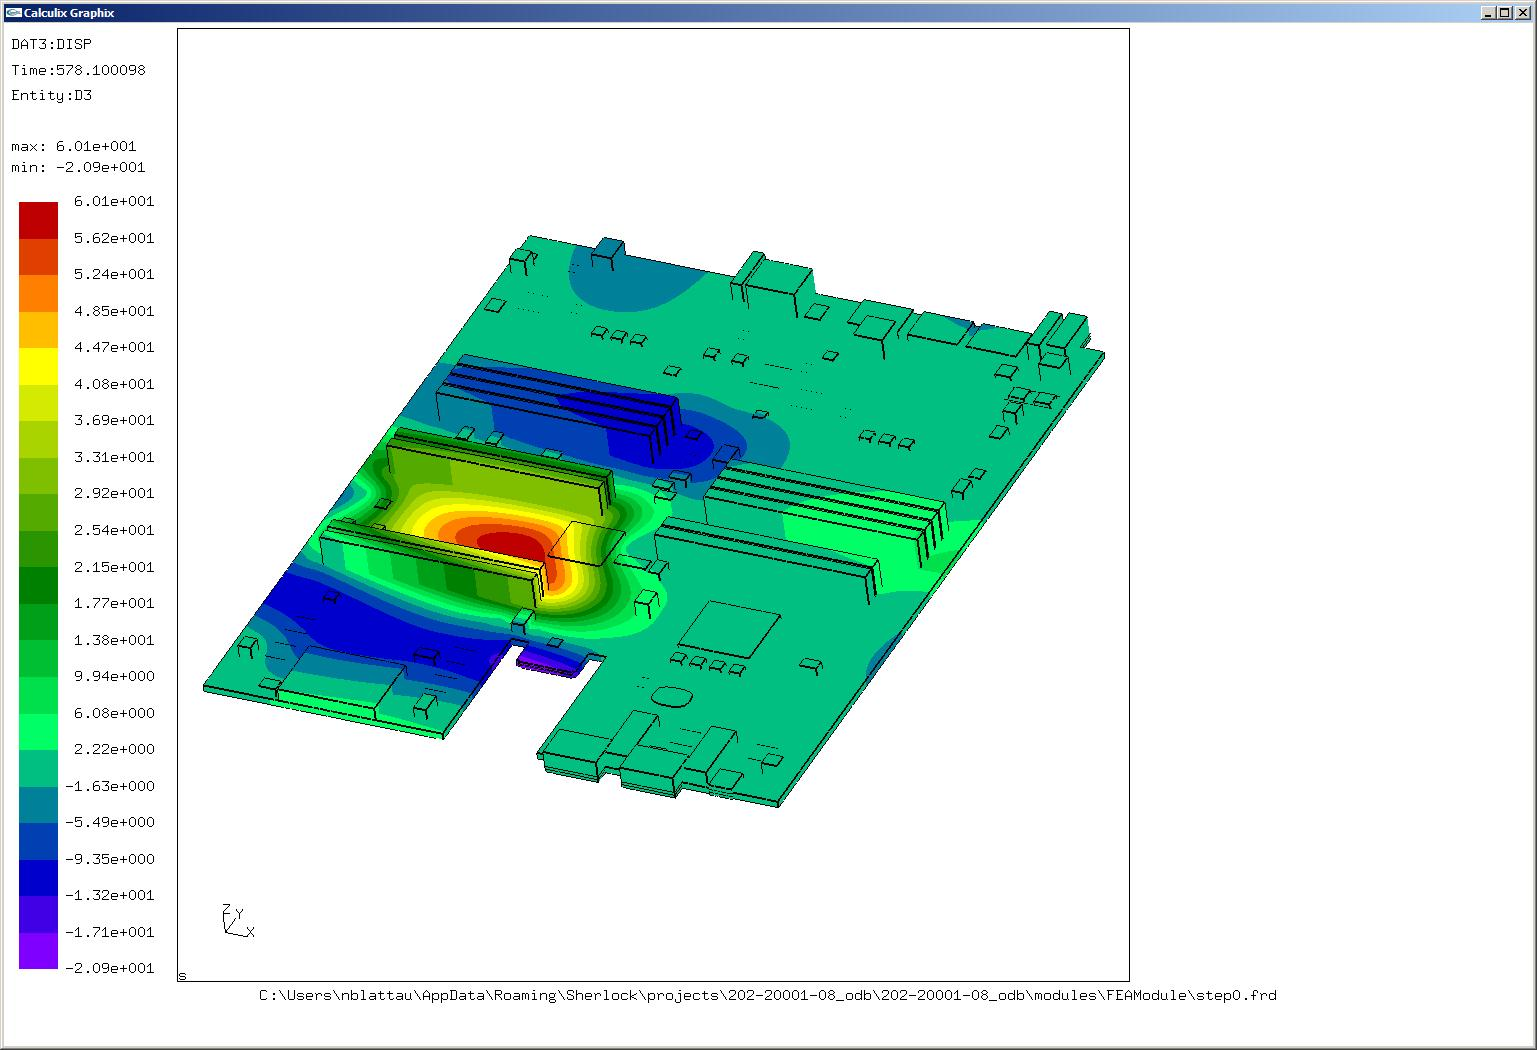
\includegraphics[width=0.56\textwidth]{feaexample}
    \centering
    \caption{The result of FEA\autocite{feaexample}}
    \centering
    \end{figure}


\section{Methodology} \label{Methodology}%700
    \subsection{Theory}\label{Theory}
    \pagebreak
    \subsection{Finite Element Analysis} \label{FEA}%338, donezo
    As explained in \ref{FEM}, FEA is a method to compute ODEs, and as shown in \ref{Theory} the resonant frequencies of the beam can be calculated with an ODE.
    Thankfully, there exists tools to calculate the FEM built-in on many CAD suites to make the calculations, in this case, PTC's Onshape is to be used.\\
    To start, we need to define the variables and constants.
    \begin{align}%eqn:constants
    \label{eqn:constants}
    \begin{split}
    \diameter&=22mm
    \\
    l_{1}&=200mm\\
    l_{3}&=150mm\\
    l_{5}&=100mm\\
    E_{1}&=5\text{ J}\\
    E_{2}&=7.5\text{ J}\\
    E_{3}&=10\text{ J}\\
    \end{split}
    \end{align}
    As shown in \eqref{eqn:constants}, The diameter $\diameter$ and length $l$ have been picked according to commonly available materials and for ease of acsess, the lengths picked should also be able to give a wide variety of frequencies.
    Additionally, the material properties of hardened carbon steel are required to run the simulation, shown in \eqref{eqn:steel}, these values were taken from Onshape.
    \begin{align}%eqn:steel
    \label{eqn:steel}
    \begin{split}
    \rho&=7.850\times10^{-6}~\frac{kg}{mm^{3}}\\
    \nu&=0.292\\
    E&=200000000000~Pa\\
    \end{split}
    \end{align}
    Where $\rho$ is the Density, $\nu$ is Poisson's ratio and $E$ is Young's Modulus
    \begin{figure}[H]%fig:VarTable
    \begin{center}
    \begin{tabular}[H]{|c||c|c|c|c|}
    \hline
    Variable & Length $l$ & Energy $E$ & Deformation $\epsilon$ & Frequency $f$ \\
    \hline\hline
    Type & Independent & Independent & Dependent & Dependent \\
    & Discrete & Discrete & Continuous & Continuous \\
    \hline
    Unit & mm & J & mm & hz, s$^{-1}$ \\
    \hline
    \end{tabular}
    \end{center}
    \caption{The Table Of Variables}\label{fig:VarTable}
    \end{figure}
    The Table of variables is as Figure \ref{fig:VarTable}, or in other words, length $l$ and energy $E$ will be changed according to \eqref{eqn:constants} and a seperate simulation will be ran for each.
    \begin{figure}[H]%fig:CADPic
    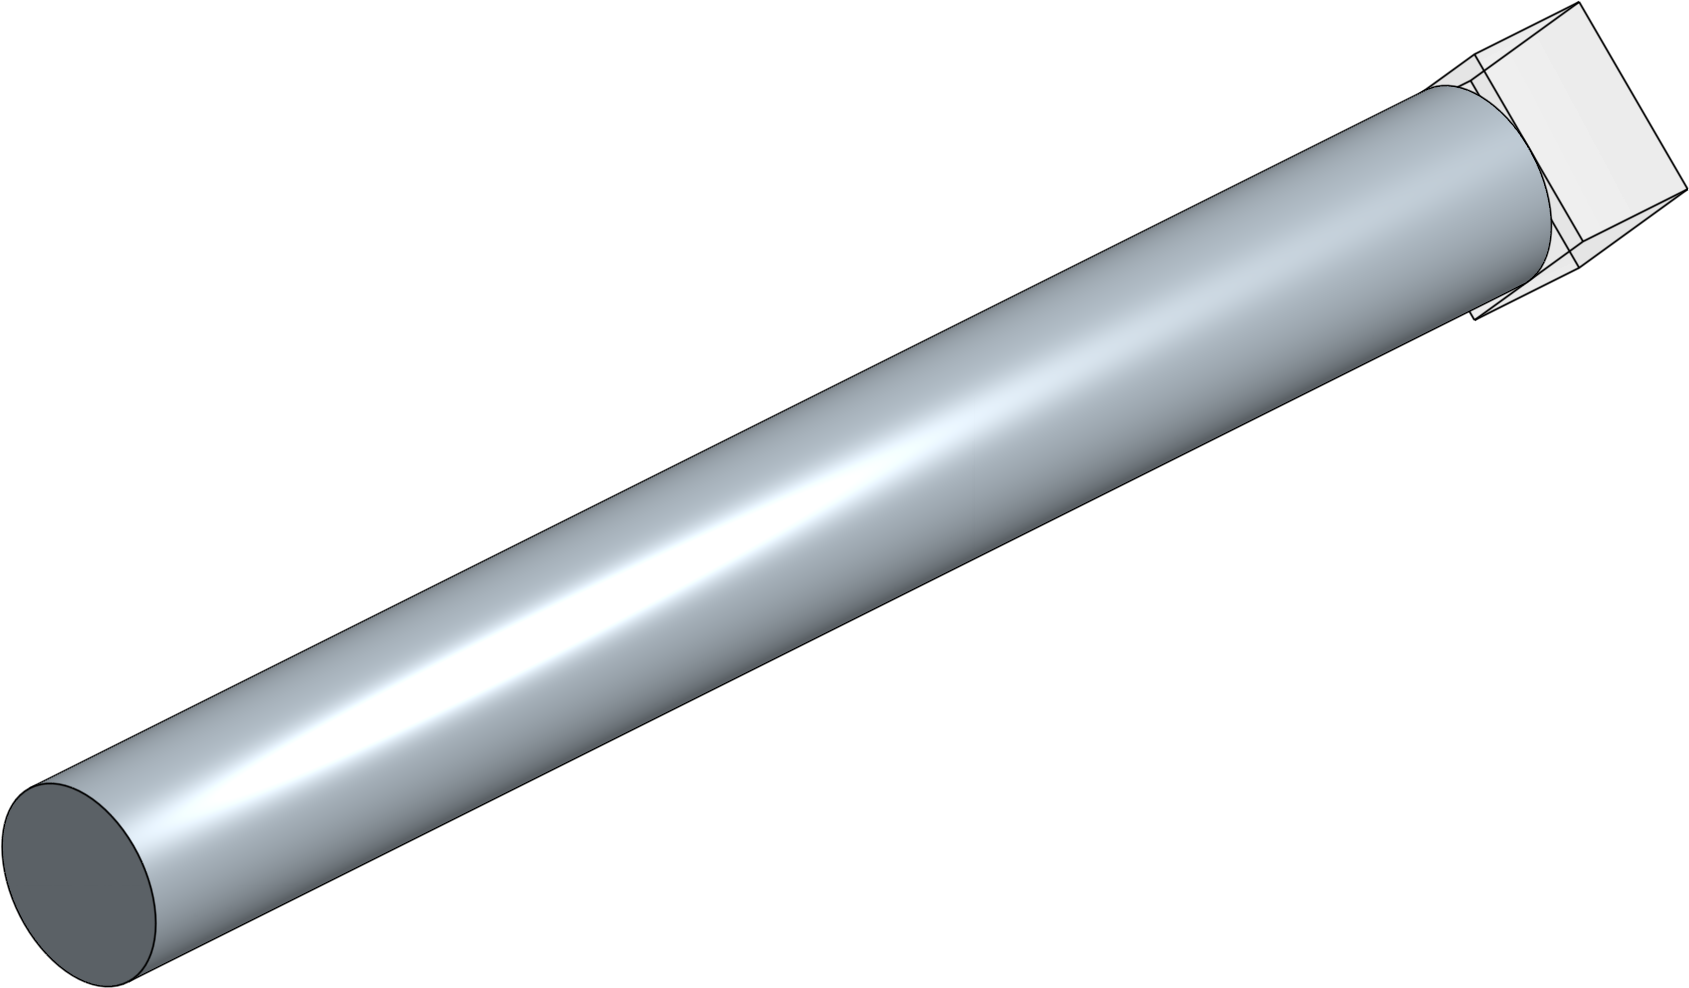
\includegraphics[width=0.5\textwidth]{CADPic}
    \centering
    \caption{The Design of the Circular beam, $\diameter=22mm$ and $l=200mm$}\label{fig:CADPic}
    \centering
    \end{figure}
    To start, a model was created for each length $l$, and was attached to a solid block as a reference frame. The 200mm long one can be seen in Figure \ref{fig:CADPic}
    And for each block, the FEA simulation was run 3 times, once per $E$ value.
    The deformation model for each model can be seen in Figure \ref{fig:FEAPic}, and the readings from the simulation was put into Figure \ref{fig:FEAtable} and as expected, inital energy $E$ shows no correlation with the frequency $f$, and the second part of \eqref{eqn:theory} has been shown true.
    \begin{figure}[H]%fig:FEAPic
    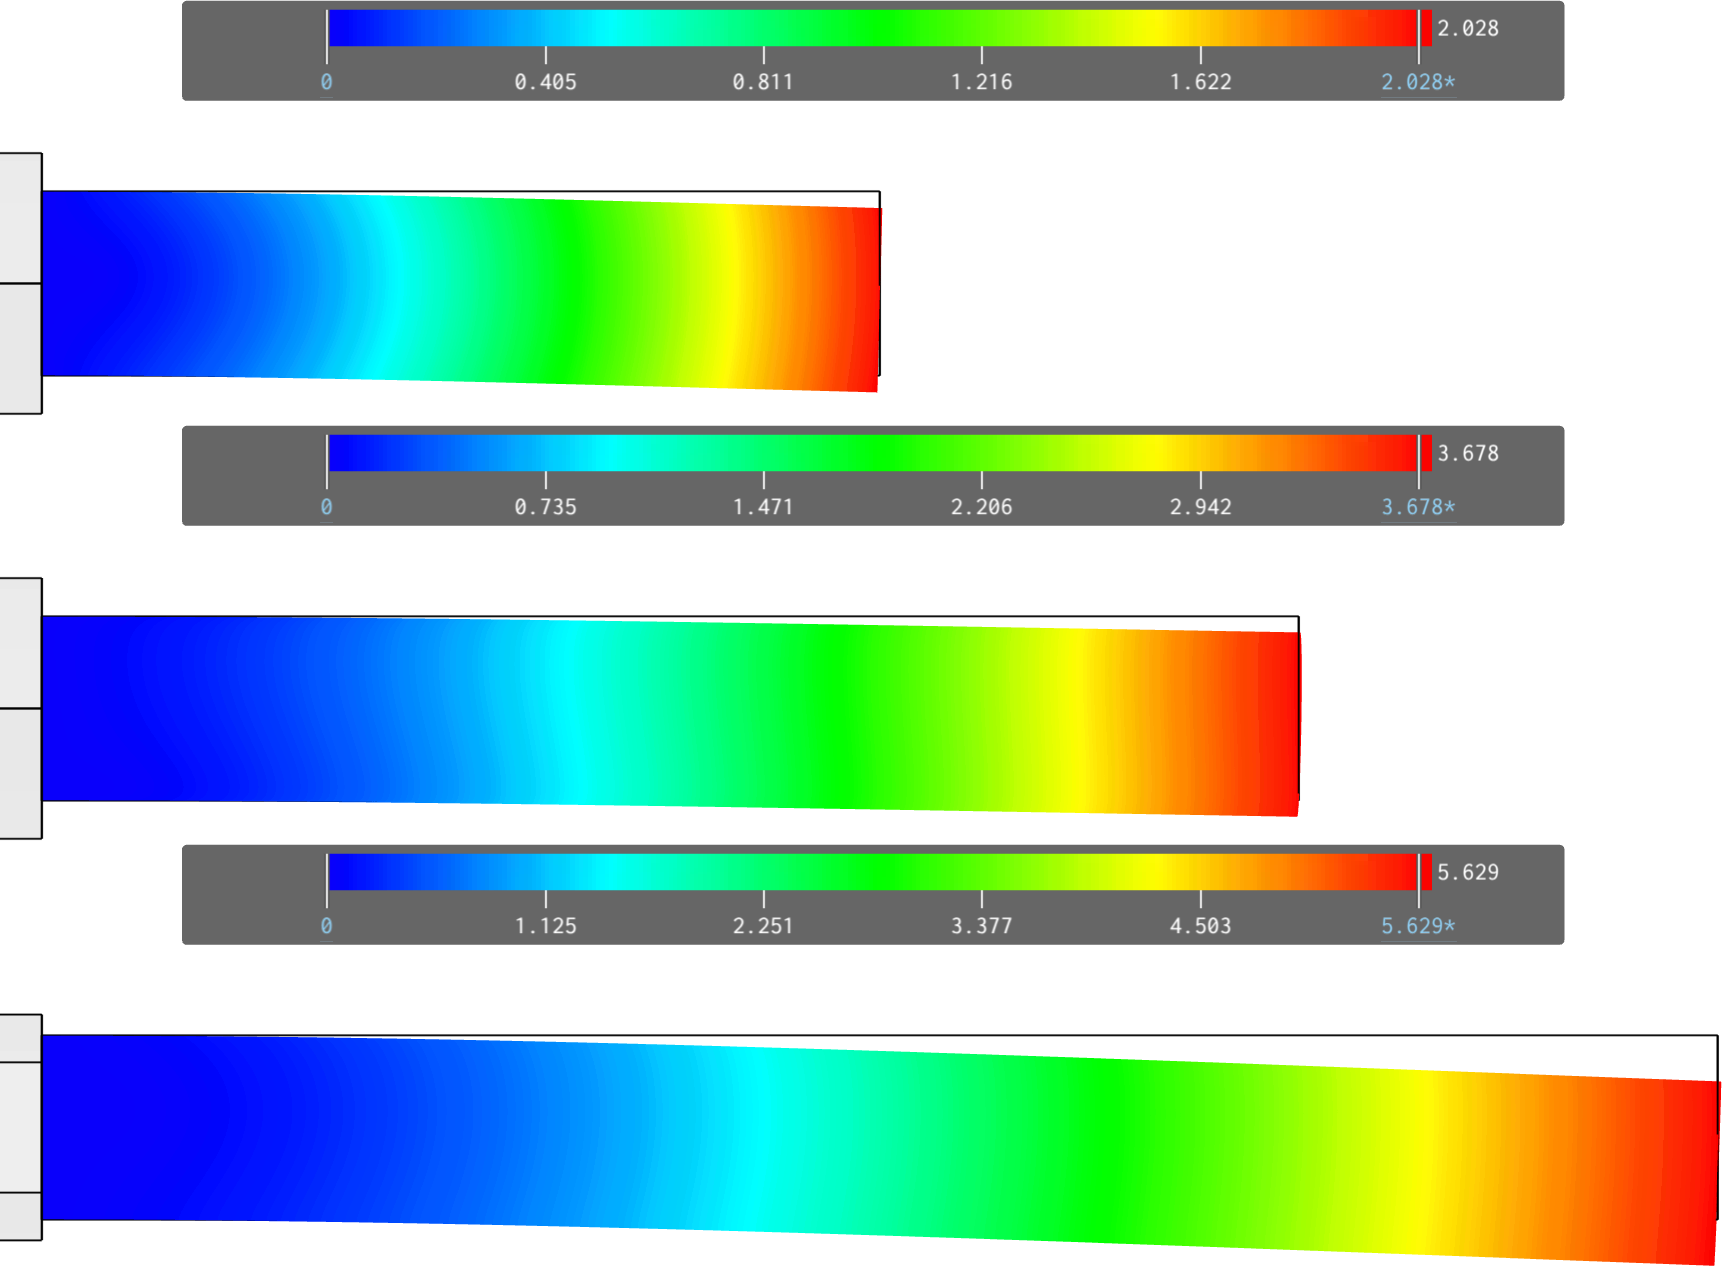
\includegraphics[width=0.7\textwidth]{FEA3}
    \centering
    \caption{The result of FEA, With the colours representing Deformation $\epsilon$ in mm.}\label{fig:FEAPic}
    \centering
    \end{figure}
    \begin{figure}[H]%fig:FEAtable
    \begin{center}
    \begin{tabular}[H]{|c|c||c|c||c|}
    \hline
    $l$ & $E$ & $f$ & $\epsilon$ & $\frac{1}{l^{2}}$\\
    \hline\hline
    100mm & 5 J & 1536 hz & 1.434 mm & $10^{-4}~mm^{-2}$\\
    \hline
    100mm & 7.5 J & 1536 hz & 1.756mm & $10^{-4}~mm^{-2}$ \\
    \hline
    100mm & 10 J & 1536 hz & 2.028mm & $10^{-4}~mm^{-2}$\\
    \hline
    150mm & 5 J & 694.2 hz & 2.601mm & $4.44\times10^{-5}mm^{-2}$\\
    \hline
    150mm & 7.5 J & 694.2 hz & 3.185mm & $4.44\times10^{-5}mm^{-2}$\\
    \hline
    150mm & 10 J & 694.2 hz & 3.678mm & $4.44\times10^{-5}mm^{-2}$\\
    \hline
    200mm & 5 J & 392.9 hz & 3.981mm & $2.5\times10^{-5}mm^{-2}$\\
    \hline
    200mm & 7.5 J & 392.9 hz & 4.876mm & $2.5\times10^{-5}mm^{-2}$\\
    \hline
    200mm & 10 J & 392.9 hz & 5.630mm & $2.5\times10^{-5}mm^{-2}$\\
    \hline
    \end{tabular}
    \end{center}
    \caption{The FEA Results}\label{fig:FEAtable}
    \end{figure}
    For the first part of \eqref{eqn:theory}, the modeling of $\frac{1}{l^{2}}$ in relation to $f$ is required, so for each value of $l$, and calculating it for each of gives the $\frac{1}{l^{2}}$ column of Figure \ref{fig:FEAtable} and the unit analysis regarding the unit of $\frac{1}{l^{2}}$ is given in \eqref{eqn:unitconv}.
    \begin{align}%eqn:unitconv
    \label{eqn:unitconv}
    \begin{split}
    \text{Given:}\\
    l&=\text{mm}\\
    f^{2}&=\text{mm}^{2}\\
    \text{Thus:}\\
    \frac{1}{f^{2}}&=\text{mm}^{-2}\\
    \end{split}
    \end{align}
    According to \eqref{eqn:theory}, $\frac{1}{l^{2}}$ and $f$ should be proportional, in other words, when graphed, the best line of fit should be a straight line crossing the origin, or in mathemacial terms, $f \approx k \frac{1}{l^{2}}$ where $k$ is arbitrary.
    \begin{figure}[H]%fig:regerssion
    \begin{center}
    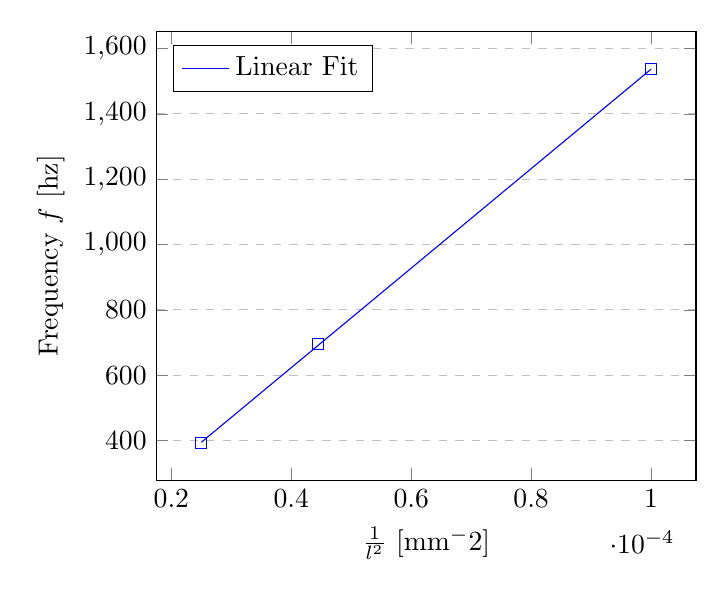
\begin{tikzpicture}
    \begin{axis}[
        xlabel={$\frac{1}{l^{2}}$ [mm$^-2$]},
        ylabel={Frequency $f$ [hz]},
        legend pos=north west,
        ymajorgrids=true,
        grid style=dashed,
    ]
    \addplot [
        domain=2.5e-5:1e-4,
        samples=100,
        color=blue,
        ]
        {15226342.949*x + 13.971};
    \addlegendentry{Linear Fit}
    \addplot+[
        only marks,
        color=blue,
        mark=square,
        ]
        coordinates {
        (1e-4,1536)(4.44e-5,694.2)(2.5e-5,392.9)
        };
    \end{axis}
    \end{tikzpicture}

    \caption{Table of ($\frac{1}{l^{2}}$,$f$) and linear regression}\label{fig:regression}
    \end{center}
    \end{figure}
    Doing the regression analysis, $f=15226342\frac{1}{l^{2}}+13.9$, or $f\propto\frac{1}{l^{2}}+9.1\times10^{-7}$ and the coefficient of determination is $R^{2}=0.99998$.\\
    While the result is offby $9.1\times10^{-7}$, this error is small enough in magnitude to be ignored.



    \subsection{Experiment}
\section{Results And Analysis}%500
    \subsection{Uncertainty Analysis}
\section{Discussion}%500
\section{Conclusion}%500

\pagebreak
\addcontentsline{toc}{section}{References}
\printbibliography


\end{document}

